\documentclass[style=sailor,size=12pt]{powerdot}
\usepackage{epic,array,ecltree,url,calrsfs}
\usepackage[nointegrals]{wasysym}
\usepackage{listings}
\usepackage{epsfig}
\usepackage{amsmath}
\usepackage{amsfonts}
\usepackage{amssymb}
\usepackage{amsxtra}
\usepackage{amsthm}
\usepackage{mlextra} % Must be below ams packages
\usepackage{mathrsfs}
\usepackage{color}
\usepackage{array}
\usepackage{graphicx}
\graphicspath{ {../art/} }
\usepackage{bm}
\usepackage{tikz}
\usepackage{multicol}
\usepackage{enumitem}

\pdsetup{method=normal}

\begin{document}

\begin{wideslide}[bm=,toc=]{Decision vs semi-decision procedure}
\begin{itemize}
\item A {\em decision procedure\/} for a set $A$ returns ``yes'' on input $x$ 
{\bf iff} $x\in A$ and ``no'' {\bf iff} $x\not\in A$.
\item A decision procedure always says ``yes'' or ``no'' on any input.
\item A {\em semi-decision\/} procedure for a set $A$ returns ``yes'' on input $x$
{\bf iff} $x\in A$ and ``no'' {\bf only if} $x\not\in A$.
\item A semi-decision procedure need not terminate on an input $x$ if $x\not\in A$.
\end{itemize}
\end{wideslide}

% ADD slide from Ben Ari 2.5.1.

\begin{wideslide}[bm=,toc=]{Decidable vs undecidable problems}
\begin{itemize}
\item A set is {\em decidable\/} iff there's a decision procedure for it.
\item A set is {\em semi-decidable\/} iff there's a semi-decision procedure for it.
\item Decidable implies semi-decidable but the converse is not true.
\item Another term for decision procedure is ``algorithm''.
\item Both propositional satisfiability (PL-SAT) and propositional validity (PL-VAL) are decidable.
\end{itemize}
\end{wideslide}

\begin{wideslide}[bm=,toc=]{A Trivially Decidable Set}
\begin{itemize}
\item Let $S$ be the set of all even length strings over $\Sigma = \{0\}$. 
\item $S$ is decidable iff there is a decision procedure for $S$.
\item That is, if and only if there is an algorithm that takes a string $x \in
\Sigma^*$ and returns \emph{yes} if $x \in S$ and \emph{no} if $x \notin S$.
\item We have already seen a machine that does this: 
\end{itemize}
\begin{figure}[h]
\centering
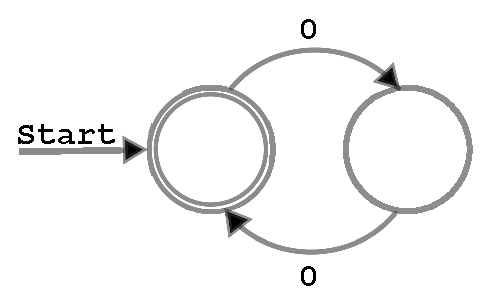
\includegraphics[width=2.5in, height=.75in,keepaspectratio=true]{evenzeroautomata.eps}
\label{2sp}
\end{figure}
To prove this is a decision procedure, you must show:
\begin{itemize}
\item It accepts all even length strings. 
\item It rejects all other strings. 
\item It always accepts or rejects (i.e.\ does not run forever).
\end{itemize}
\end{wideslide}

\begin{wideslide}[bm=,toc=]{The Halting Problem as an Example of a Semi-Decidable Set}
\begin{itemize}
\item Let $M$ be a string that represents a well-formed computer program.
\item That is, $M \in P$, where $P = \{M \in \Sigma^* | M \text{ is a well-formed 
  program}\}$.
\item Let $w \in \Sigma^*$ be a string that represents some input to the program.
\item Now let $(M,w)$ be a string that represents a pairing of a program and an
input, and define the language $H$ as follows:\\ 
$H = \{(M,w) \in \Sigma^* | \text{ the program } M
\text{ eventually halts when run on input } w\}$.
\item Clearly, we can create a procedure that always says \emph{yes} when given a
string $(M,w) \in H$. 
\item We can also create a procedure that will say \emph{no} only if $(M,w) \notin H$.
\item But there is no procedure that will always say \emph{no} if $(M,w) \notin H$
\end{itemize}
\end{wideslide}

\begin{wideslide}[bm=,toc=]{Decision Procedures in Propositional Logic}
\begin{defn}{2.40}[Ben Ari]
Let $\mathcal{U} \subseteq \mathcal{F}$ be a set of formulas. An algorithm
is a \emph{decision procedure} for $\mathcal{U}$ if given an arbitrary formula
$A \in \mathcal{F}$, it terminates and returns the answer \emph{yes} if
$A \in \mathcal{U}$ and the answer \emph{no} if $A \notin \mathcal{U}$.
\end{defn}
\begin{itemize}
\item Let $\mathcal{U}$ be the set of decidable formulas. Then a decision
procedure for $\mathcal{U}$ is called a decision procedure for satisfiability.
\item Similarly, if $\mathcal{U}$ is the set of valid formulas, a decision
procedure for $\mathcal{U}$ is a decision procedure for validity. 
\end{itemize} 
\end{wideslide}

\begin{wideslide}[bm=,toc=]{Refutation Procedures}
Recall \textbf{Theorem 2.39}: $A$ is valid if and only if $\ngg A$ is unsatisfiable.
$A$ is satisfiable if and only if $\ngg A$ is falsifiable.
\begin{itemize}
\item Therefore, a decision procedure for satisfiability can be used as a
decision procedure for validity: 
\begin{itemize}
\item To decide if $A$ is valid, apply decision procedure for satisfiability to $\ngg A$. 
\end{itemize} 
\item This type of decision procedure is called a ``refutation procedure.'' 
\item Can be more efficient---only need to find a single counterexample.
\end{itemize} 
\end{wideslide}

\begin{wideslide}[bm=,toc=]{Examples of Decision Procedures for Satisfiability
  of Formulas in Propositional Logic}
\begin{itemize}
\item Enumerate the truth table (requires $2^n$ entries for $n$ literals).
\item Two alternate algorithms:
\begin{itemize}
\item Resolution procedure / propositional resolution.
\item Davis--Putnam--Logemann--Loveland (DPLL) algorithm (also gives a model if
    the formula is satisfiable).
\end{itemize} 
\item Both resolution and DPLL are nondeterministic. 
\item We will introduce resolution here, and later review the explanation of DPLL
given by Almeida.
\end{itemize} 

\end{wideslide}

\begin{wideslide}[bm=,toc=]{Resolution Overview}
Resolution is a refutation procedure to check whether a formula is
unsatisfiable.\\
~\\
{\bf \underline{Strategy:}}\\
\begin{enumerate}
\item Convert a formula, $A$, to \emph{clausal form} (producing a set of clauses $S$).
\item Apply the resolution rule to $S$ to produce an equisatisfiable set of
clauses.
\item Continue until:
\begin{enumerate}
\item The resolution rule cannot be further applied, or
\item An unsatisfiable clause is produced.
\end{enumerate}
\end{enumerate}
Since the resolution rule preserves satisfiability, the production of an
unsatisfiable clause indicates the original formula was unsatisfiable.
\end{wideslide}

\begin{wideslide}[bm=,toc=]{Clausal Form}
Clausal form is a notational variant of CNF.
\begin{itemize}
\item Convenient for describing resolution and DPLL.
\end{itemize}

\begin{defn}{4.5}[Ben Ari]
\end{defn}
\vspace*{-3ex}
\begin{itemize}
\item A \emph{clause} is a set of literals.  
\item A clause is considered to be an implicit disjunction of its literals.
\item A \emph{unit clause} is a clause consisting of exactly one literal.
\item The empty set of literals is the \emph{empty clause}, denoted by $\Box$.
\item A formula in \emph{clausal form} is a set of clauses.
\item A formula is considered to be an implicit conjunction of its clauses.
\item The formula that is the \emph{empty set of clauses} is denoted by
$\emptyset$.
\end{itemize}

The significant difference: now using sets instead of trees.
\begin{itemize}
\item This works because of the properties of CNF. 
\end{itemize}
\end{wideslide}

\begin{wideslide}[bm=,toc=]{Clausal Form Example}
\begin{ex}{4.7}
The CNF formula:
\[ (p \lor r)\land (\ngg q \lor \ngg p \lor q) \land (p \lor \ngg p \lor q) \] is
logically equivalent to its clausal form:
\[ \{\{p,r\},\{\ngg q, \ngg p, q\},\{p, \ngg p, q\} \} \]
\end{ex}
\end{wideslide}

\begin{wideslide}[bm=,toc=]{Trivial Clauses, Empty Clauses and the\\ Empty Set of
  Clauses}
\begin{defn}{4.8}
A clause is \emph{trivial} if it contains a pair of clashing literals.
\end{defn}
\begin{lem}{4.9}
Let $S$ be a set of clauses and let $C \in S$ be a trivial clause. Then $S -
\{C\}$ is logically equivalent to $S$.
\end{lem}
\begin{lem}{4.10}
$\Box$, the empty clause, is unsatisfiable. $\emptyset$, the empty set of
clauses, is valid.
\end{lem}
\begin{itemize}
\item Recall that a clause is satisfiable iff there is \emph{some} interpretation
under which \emph{at least one literal} in the clause is true.
\begin{itemize}
\item The empty clause, $\Box$, contains no literals, so therefore no literals with a value of T.
\end{itemize}
\item A set of clauses is valid iff \emph{every} clause in the set is true in
\emph{every} interpretation.
\begin{itemize}
\item There are no clauses in $\emptyset$, so this is vacuously true.
\end{itemize}
\end{itemize}

\end{wideslide}

\begin{wideslide}[bm=,toc=]{Clausal Form: Additional Notation}
\begin{itemize}
\item Set delimiters are removed from each clause.
\item Negated literals are denoted by a bar over the literal.
\item Example: \[ \{\{p,r\},\{\ngg q, \ngg p, q\},\{p, \ngg p, q\} \} \] is
written as:
\[\{pr, \bar{q}\bar{p}q, p\bar{p}q \}  \]
\item $S$ is a formula in clausal form, $C$ is a clause and $l$ is a literal.
\item If $l$ is a literal, $l^c$ is its complement.
\item Example: if $l = p$ then $l^c = \bar{p}$. If $l = \bar{p}$ then $l^c = p$.
\end{itemize}
\end{wideslide}

\begin{wideslide}[bm=,toc=]{Resolution Rule}
Let $C_1, C_2$ be clauses such that $l \in C_1$, $l^c \in C_2$. The clauses
$C_1,C_2$ are said to be clashing clauses and to clash on the complementary
pair of literals $l,l^c$. $C$, the resolvent of $C_1$ and $C_2$, is the
clause:\\
\[ 
  Res(C_1,C_2) = (C_1 - \{l\}) \cup (C_2 - \{l^c\})
\]
\begin{ex}{4.15}[Ben Ari]
The pair of clauses $C_1 = ab\bar{c}$ and $C_2 = bc\bar{e}$ clash on the pair
of complementary literals $c, \bar{c}$. The resolvent is:

\[ 
  C = (ab\bar{c} - \{\bar{c}\}) \cup (bc\bar{e} - \{c\}) = ab\cup b\bar{e} = ab\bar{e}
  \]

\end{ex}
\begin{thm}{4.17}
The resolvent $C$ is satisfiable if and only if the parent clauses $C_1$ and
$C_2$ are both satisfiable.
\end{thm}

\end{wideslide}

\begin{wideslide}[bm=,toc=]{Clauses that Clash on More Than One Literal}
\begin{lem}{4.16}[Ben Ari]
If two clauses clash on more than one literal, their resolvent is a trivial
clause.
\end{lem}
{ \bf \underline{Intuition}}\\
Consider the following pair of clauses:
\[
  \{l_1, l_2\} \cup C1,  \{l_1^c, l_2^c\} \cup C2
  \]
Now perform resolution on $\{l_1, l_1^c\}$: 
\[
  (\{l_1, l_2\} \cup C1 - \{l_1\})\cup (\{l_1^c, l_2^c\} \cup C2 - \{l_1^c \})
\]
\[
  = (\{l_2\} \cup C1) \cup (\{l_2^c\} \cup C2)
\]
\[
  = \{l_2, l_2^c\} \cup C1 \cup C2
\]
Note that the resolvent is a trivial clause.
\end{wideslide}

\begin{wideslide}[bm=,toc=]{The Resolution Procedure}
{ \bf Input:} A set of clauses $S$.\\
{ \bf Output:} $S$ is satisfiable or unsatisfiable.\\
\begin{enumerate}
\item Let $S$ be a set of clauses and define $S_0 = S$.
\item Repeat the following steps to obtain $S_{i+1}$ from $S_i$ until
the procedure terminates.
\begin{enumerate}
\item \emph{Choose} a pair of clashing clauses $\{C_1,C_2\} \subseteq S_i$ that
has not been chosen before.
\item Compute $C = Res(C_1,C_2)$ according to the resolution rule.
\item If $C$ is not a trivial clause, let $S_{i + 1} = S_i \cup \{C\}$;
otherwise, $S_{i+1} = S_i$.
\end{enumerate}
\end{enumerate}
Terminate the procedure if:
\begin{itemize}
\item $C = \Box$.
\item All pairs of clashing clauses have been resolved. 
\end{itemize}

\end{wideslide}

\begin{wideslide}[bm=,toc=]{Resolution Example}
\begin{ex}{4.19}
Consider the set of clauses:
\[
  S  = S_0 = \{p,\bar{p}q,\bar{r},\bar{p}\bar{q}r\}
  \]
\end{ex}
\begin{enumerate}
\item $Res(\bar{r},\bar{p}\bar{q}r) = \bar{p}\bar{q}$, which is not trivial.
\item $S_1  = \{p,\bar{p}q,\bar{r},\bar{p}\bar{q}r, \bar{p}\bar{q}\}$
\item $Res(\bar{p}q,\bar{p}\bar{q}) = \bar{p}$, which is not trivial.
\item $S_2  = \{p,\bar{p}q,\bar{r},\bar{p}\bar{q}r, \bar{p}\bar{q}, \bar{p}\}$
\item $Res(p,\bar{p}) = \Box $, so we are finished.
\end{enumerate}
{\bf Conclusion:} $S$ is unsatisfiable.\\
~\\
Note that the algorithm must \emph{choose} which clauses to resolve.
\end{wideslide}

\begin{wideslide}[bm=,toc=]{Figure 4.1: Resolution refutation as a tree}
\unitlength=1.0pt
\begin{center}
\begin{picture}(200,140)
\put(130,140){
  \put( -10,   0){\makebox(20,10){$\Box$}}
  \put( -70, -40){\makebox(20,10){$\bar{p}$}}
  \put(  50, -40){\makebox(20,10){$p$}}
  \put(-110, -90){\makebox(20,10){$\bar{p}\bar{q}$}}
  \put( -30, -90){\makebox(20,10){$\bar{p}q$}}
  \put(-130,-140){\makebox(20,10){$\bar{p}\bar{q}r$}}
  \put(- 90,-140){\makebox(20,10){$\bar{r}$}}
  \put(   0,   0){\line(-2,-1){58}}
  \put(   0,   0){\line( 2,-1){58}}
  \put( -60, -40){\line(-1,-1){38}}
  \put( -60, -40){\line( 1,-1){38}}
  \put(-100, -90){\line(-1,-2){18}}
  \put(-100, -90){\line( 1,-2){18}}
}
\end{picture}
\end{center}
\end{wideslide}

\begin{wideslide}[bm=,toc=]{Measuring Complexity}
We measure the difficulty of a problem by the resources (time and space)
  required by some optimal machine that solves the problem.
\begin{itemize}
\item The time and space used are measured against input size.
\item A Turing Machine is the most commonly used model. 
\end{itemize}
\begin{defn}{}[Hopcroft et al]
A Turing Machine $M$ is said to be of \emph{time complexity} $T(n)$ [or to have
``running time $T(n)$''] if whenever $M$ is given an input $w$ of length
$n$, $M$ halts after making at most $T(n)$ moves...
\end{defn}
\begin{itemize}
\item Ex: if $T(n) = kn$ for some constant $k$, the problem is solvable in
\emph{linear} time.
\item Ex: if $T(n) = an^k + bn^{k-1}... + c$ the algorithm is solvable in polynomial
time.
\end{itemize}
\end{wideslide}

\begin{wideslide}[bm=,toc=]{Intuition for Deterministic and nondeterministic Machines}
\begin{itemize}
\item A deterministic machine makes one ``decision'' at a time.
\item A non-deterministic machine makes all possible decisions at the same a time.
\end{itemize}
{\bf Deterministic Program Example:} Consider a program navigating a maze. 
\begin{itemize}
\item When it reaches a fork, it must choose a single direction to explore.
\item Later, it can come back and try other directions. 
\item However, it can only test one at a time.
\end{itemize}

{\bf Nondeterministic Program Example:} A nondeterministic program in a maze. 
\begin{itemize}
\item Whenever a nondeterministic program reaches a fork, it can explore all
directions at the same time. 
\item As if making copies of itself. 
\item The copy that finds the exit of the maze returns the answer.
\item The other copies die off. 
\item The effect is as though the machine always guesses the best choice.
\end{itemize}

\end{wideslide}

\begin{wideslide}[bm=,toc=]{P and NP}
\begin{itemize}
\item $P$ and $\mli{NP}$ are classes of problems (i.e. languages).
\item $P$ stands for polynomial and $\mli{NP}$ stands for nondeterministic
polynomial.
\end{itemize}
\begin{defn}{}[Hopcroft et al]
We say a language $L$ is in class $P$ if there is some polynomial $T(n)$ such
that $L = L(M)$ for some deterministic $\mli{TM}$ $M$ of time complexity
$T(n)$. 
\end{defn}

\begin{defn}{}[Hopcroft et al]
A language $L$ is in the class $\mli{NP}$ (nodeterministic polynomial) if there
is a nondeterministic $\mli{TM}$ $M$ and a polynomial time complexity $T(n)$
such that $L = L(M)$, and when $M$ is given an input of length $n$, there are
no sequences of more than $T(n)$ moves of $M$.
\end{defn}
Observe that the above definitions imply $P \subseteq \mli{NP}$.
\end{wideslide}

\begin{wideslide}[bm=,toc=]{NP and coNP}
\begin{itemize}
\item Consider $(p\vee\neg q)\wedge(\neg p\vee q)$.
\item It is satisfiable ($p=q=T$ or $p=q=F$).
\item A nondeterministic algorithm can {\em guess\/} an interpretation and then {\em verify\/}
it satisfies the formula in time linear in the formula's length.
\item Guessing takes time linear in the number of propositional variables.
\item Hence it's possible to decide satisfiability of any propositional formula {\em nondeterministically\/}
in time proportional to its length.
\item Hence PL SAT belongs to NP, the class of problems 
solvable in Nondeterministic Polynomial time.
\item coNP is the complement of the class NP.
\item PL-UNSAT is in coNP (not in NP unless NP=coNP).
\end{itemize}
\end{wideslide}


\begin{wideslide}[bm=,toc=]{NP and coNP completeness}
\begin{itemize}
\item Widely conjectured, though unproven, NP contains problems that cannot be solved deterministically
in polynomial time.
\item There's a class of problems in NP, called NP-complete.
\item Any NP-complete problem that can be solved in deterministic polynomial time implies {\em every\/}
problem in NP can be solved in deterministic polynomial time.
\end{itemize}
\end{wideslide}

\begin{wideslide}[bm=,toc=]{Two Alternative Possibilities for Relating Algorithm
  Classes P, NP, NP-Complete and NP-Hard}

\begin{figure}[h]
\centering
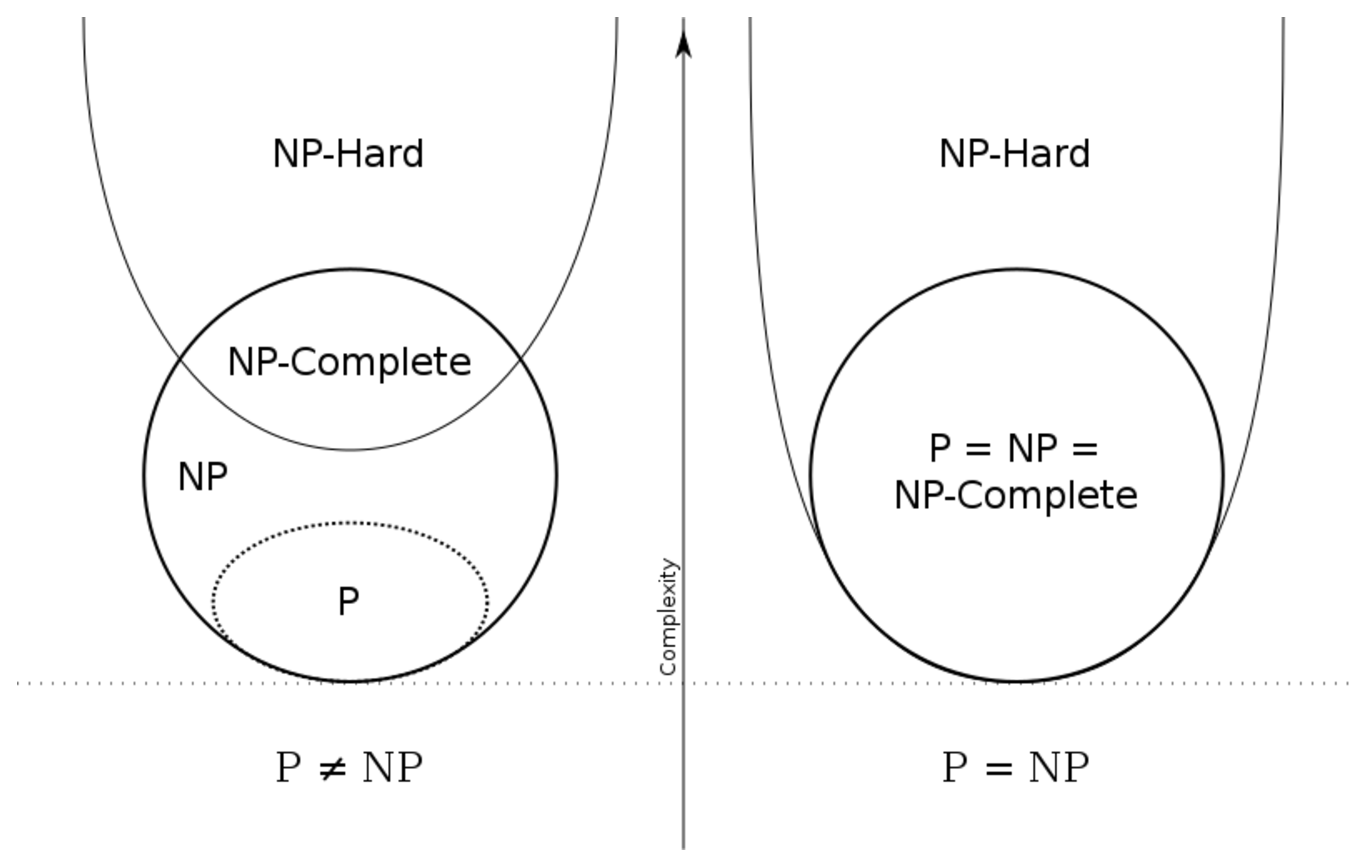
\includegraphics[width=4in, height=4in,keepaspectratio=true]{np_np-complete_np-hard.eps}
\label{2sp}
\end{figure}
By Behnam Esfahbod, CC BY-SA 3.0, \url{https://commons.wikimedia.org/w/index.php?curid=3532181}
\end{wideslide}

\begin{wideslide}[bm=,toc=]{Intuition for Reduction}
We say a problem $A$ \emph{reduces} to another problem $B$ if any algorithm that
solves problem $B$ can also be used to solve problem $A$.
\begin{itemize}
\item That is, solving $B$ is sufficient to solve both $A$ and $B$.
\item Informally, solving $B$ must be at least as hard as $A$, or harder.
\item Notation: $A$ reduces to $B$ is written $A \leq B$.
\end{itemize}
Note this definition implies that a problem generally \emph{reduces} to a
\emph{harder} problem, in contrast to what you might expect the word
\emph{reduce} to mean.
\\~\\
More formally: 
\vspace{-2ex}
\begin{defn}{}[\url{https://en.wikipedia.org/wiki/Many-one_reduction}]
Suppose $A$ and $B$ are formal languages over the alphabets $\Sigma$ and $\Gamma$, 
respectively. A many-one reduction from $A$ to $B$ is a total computable function 
$f : \Sigma^* \to \Gamma^*$ that has the property that each word $w$ is in $A$ if and only 
if $f(w)$ is in $B$ (that is, $A=f^{-1}(B)$).
\end{defn}
\end{wideslide}

\begin{wideslide}[bm=,toc=]{NP and coNP completeness}
\begin{itemize}
\item PL-SAT is NP complete (proofs due to Cook and Levin).
\item The complement of an NP-complete problem is coNP complete.
\item Hence PL-UNSAT is coNP complete.
\item PL-UNSAT many-one reduces to PL-VAL in polynomial time.
\item Hence PL-VAL is coNP hard.
\item PL-INVAL (find a falsifying interpretation) is in NP and therefore PL-VAL is in coNP.
\item Thus PL-VAL is coNP complete.
\item PL-VAL is harder than PL-SAT; not in NP unless NP = coNP which is unlikely.
\item Things change in FOL: FOL-SAT becomes harder than FOL-VAL!
\end{itemize}
\end{wideslide}

\end{document}
